\section{THE DETAILS}
\label{sec:details}
In section \ref{sec:appr} we propose a local watermarking algorithm, which
can insert watermark according to the local information. In this section, we 
will introduce our approach in details and finally preform some reliability 
analysis. Before introducing the algorithms, we have to specify some 'Input'
and 'Output' notions, which will appear in the following algorithms.

\begin{algorithm}[h]
\begin{algorithmic}[1]
\State 	   G: Secret grid frame
\State     S: Input dataset
\State     l: Secret square side length
\State     m: Total road segment length inside a lowest level region
\State     k: A random table served as secret hash key
\State     PO: Subregion List of Partition
\State     V : Watermarked dataset
\end{algorithmic}
\end{algorithm}

\subsection{GIS Space Partitioning Algorithm}

We first illustrate the space partition sub-function. Since the algorithm 
needs to insert the watermarks relying on just local information,
we should partition the digital road map into small regions. Ohbuchi's method 
\cite{OhbuchiUE02} partitions the space of the digital map into rectangles 
such that every rectangle contains almost equal node numbers. However, this
method is not suitable to solve the problem of "massive chop".The accuracy 
of maps of the same area from different companies varies a lot. If taking Ohbuchi's
method, we can not guarantee the partition results of insertion and detection could 
be the same. Our method is the partition the space according to the road length in 
the map area, because the road length of an area could not be changed arbitrarily. 
Even though a suspicious map consists of parts from different maps, our method still
could get almost the same partition results.


Algorithm \ref{Partition} gives the algorithm. First of all, a secret grid frame is 
persevered as a secret key of the watermarking algorithm to help the algorithm find 
the regions that completely cover the original digital road map dataset S and insert 
them into a region list. Then each region in the region list, is partitioned iteratively 
according to the density of roads such that finally the total road length included in every
subregion in which we need to insert a watermark bit has more than m meters and less than 
$4 * m$ meters. Finally, we output all of these subregions.

\begin{algorithm}[h]
\caption{Partition The Map with Quadtree}
\label{Partition}
\begin{algorithmic}[1]

\Procedure{PARTITION}{G,S}
\State Clear region list L
\State Impose secret grid frame G on space
\State Select smallest regions R0 from grid frame G that completely cover S
\State Insert R0 into region list L
\While{L is not empty}
\State Take one region R from L
\State Partition R into 4 equal size squares
\If{length of road segments in one subregion has more than $4*m$ miles}
\State Insert it into L
\Else{}
\State Insert it into PO
\EndIf
\EndWhile
\EndProcedure
\end{algorithmic}
\end{algorithm}


\subsection{Watermark Inserting Algorithm}
Algorithm \ref{Insertion} gives the watermark insertion algorithm. First
we generate a set of secret subregions. Then we select the
data points closest to the center of subregions to watermark.
In the following, we use a square centered at selected data
points to create road segments around these selected data
points and summarize the length of these road segments.
Finally we hash the length, using a secret random table, to a specific integer that is the
position to be changed and set the value of this position for
the selected data point to be 1.Like figure \ref{fig:13} illustrates.

\begin{figure}[h]
\centering
\epsfig{file=insertion.eps,width=0.6\columnwidth}
\caption{Insertion Strategy}
\label{fig:13}
\end{figure} 


\begin{algorithm}[h]
\caption{Insert Watermark Into a Map}
\label{Insertion}
\begin{algorithmic}[1]

\Procedure{INSERTION}{V,S,G,l,m}
\State PO=PARTITION( G,S )
\For{Every region ${R}_{i}$ in PO}
\If {Total length of roads in ${R}_{i}$ > $m$ miles}
\State Select point P closest to the center of ${R}_{i}$
\State Draw a square Q of side length $l$ centered at P
\State Calculate total number $sn$ of line segments intersecting Q
\State j = Hash( k,sl )
\State Set the $jth$ LSB of P to 1
\EndIf
\EndFor
\EndProcedure
\end{algorithmic}
\end{algorithm}


\subsection{Watermark Detection Algorithm}
Algorithm \ref{Detection} shows the watermark detection algorithm. 
Firstly we partition the dataset of the digital map that may have
been attacked and select the data points to be detected.
Then we calculate the total length of neighbourhood road
segments and choose the possibly watermarked bit position
in the same way as in the insertion algorithm. While selecting points,
we construct the Quadtree which depicts the whole digital map
in a hierarchy structure. For leaf nodes of the Quadtree, if the bit value at 
position we found is 1, we sign this subregion as "match". 


\begin{algorithm}[h]
\caption{Detect Watermark from a Suspicious Map}
\label{Detection}
\begin{algorithmic}[1]
\Procedure{DETECTION}{S,G,l,m}
\State PO=PARTITION( G,S )
\For{Every region ${R}_{i}$ in PO}
\If {Total length of roads in ${R}_{i}$ > $m$ miles}
\State Select point P closest to the center of ${R}_{i}$
\State Draw a square Q of side length $l$ centered at P
\State Calculate sum $sl$ of line segments intersecting Q
\State j = Hash( k,sl )
\State Set the $jth$ LSB of P to 1
\State Mark ${R}_{i}$ as "MATCH"
\State MARK\_QUADTREE( T )
\State DF\_TRAVERSE( T )
\EndIf
\EndFor
\EndProcedure
\end{algorithmic}
\end{algorithm}


It is obvious that the strategy of detection is similar to insertion. The algorithm
partitions the data source into small subregions and decide whether the very position
of point P was set to be '1'. After that we will obtain a Quadtree and get the knowledge 
that whether its leaf nodes are 'match' or not. However, since what we want is to detect
largest region that is watermarked, we have to mark the whole Quadtree.Here we implement 
a function MARK\_QUADTREE(T).The non-leaf nodes are marked to find out those suspicious 
subregions according to leaf nodes. For each node of Quadtree, we set two parameters,
'total' and 'match',which represent the total number of leaf nodes of his children and the
number of them who matches.

\begin{algorithm}[h]
\begin{algorithmic}[1]
\Statex
\Function{MARK\_QUADTREE}{$T$}
\If{ T isn't a leaf node}
\For{Each child of T:${T}_{i}$}
\State MARK\_QUADTREE(${T}_{i}$)
\State T.match+=${T}_{i}$.match
\State T.total+=${T}_{i}$.total 
\EndFor
\Else{}
\If{The region of T is "MATCH"}
\State T.match=1
\Else{}
\State T.match=0
\EndIf
\State T.total=1
\EndIf
\EndFunction
\end{algorithmic}
\end{algorithm}

Finally, we calculate the ratio of the number of leaf nodes that "match" to the total number 
of leaf nodes of this subregion. If this ratio is greater than the pre-specified threshold, 
we may conclude that the digital road map was taken from our original map. We can illustrate
this method with Figure \ref{fig:14}. Assuming that the shadow parts of sub-figure 'a' is 
cropped from the watermarked map, we can finally get a corresponding Quadtree like sub-figure 'b'.
Then we can conclude the illegal usage of the map.

\begin{figure}[h]
\centering
\epsfig{file=detection.eps,width=\columnwidth}
\caption{Detection Strategy}
\label{fig:14}
\end{figure} 

\begin{algorithm}[h]
\begin{algorithmic}[1]
\Statex
\Function{DF\_TRAVERSE}{$T$}
\State Calculate the probability of T by $P = matched/total$
\If{ P > threshold}
\State Output this region
\Else{}
\For{Each child of T:${T}_{i}$}
\State DF\_TRAVERSE(${T}_{i}$)
\EndFor
\EndIf
\EndFunction
\Statex
\end{algorithmic}
\end{algorithm}


Since we partition the target map according the density of roads and to keep the usability of map, 
the information of road length could not be changed arbitrarily changed, we have a good reason to 
assume that the result of partition will be almost the same with the insertion part. And when we 
get the same partition result, we could find the possible points which is inserted with watermarks.
Even when the map is a "mixture" of different parts from various maps and only one part of it is ours.


\subsection{Probability of Detection Accuracy}
Since those data points we select to insert watermark may originally be "1" at the
 specified position, we have to take the "False Positive Probability" into
 consideration. The insertion algorithm selects the watermarking points according
 to density of roads, thus we have a good reason the assume that the probability of
 specified bit value of a target point to be "1" is 50\%. And it is independent for
 different points. In this case, the False Positive Probability can be defined as:

\begin{equation}
{ P }_{ err }={ C }_{ N }^{ n }{ ({ 1 }/{ 2 }) }^{ N-n }{ ({ 1 }/{ 2 }) }^{ n }
\end{equation}

while $N$ is the total number of leaf nodes in the very branch and $n$ is the number of leaf nodes which match. 
So when detecting that the probability of a subregion is cropped from the watermarked map is larger than the predefined threshold, we could conclude that this subregion is a copy.

%%% Local Variables:
%%% mode: latex
%%% TeX-master: "paper"
%%% End:
